\documentclass[12pt]{article}

\usepackage[utf8]{inputenc}
\usepackage[T1]{fontenc}
\usepackage[spanish,mexico]{babel}
\usepackage{graphicx}
\usepackage[a4paper,margin=2.5cm]{geometry}
\usepackage{lmodern}
\usepackage{ragged2e}

\begin{document}
\thispagestyle{empty}

\begin{center}

\includegraphics[width=1\textwidth]{encabezado_utvam.png}
\vspace{0.3cm}
{\small CÁLCULO IV}
\end{center}

\vspace{3cm}
\begin{center}
{\Large \textbf{Funciones escalares de varias variables}}
\end{center}

\vspace{1.9cm}
\begin{center}
{\large E.D. 1.1. Ejercicios}
\end{center}

\vspace{3cm}

\begin{center}
{\small \textbf{INTEGRANTES DEL EQUIPO:}}
\end{center}

\vspace{0.1cm}
\begin{center}
{\small 253110061 - López Lemus Glynnes Eileen}
\end{center}

\vspace{0.1cm}
\begin{center}
{\small 253110509 - Rodriguez Martinez Carlos Eduardo}
\end{center}

\vspace{0.1cm}
\begin{center}
{\small 253110366 - Salinas Sanchez Javier}
\end{center}

\vspace{0.1cm}
\begin{center}
{\small 253110017 - Roque Ubaldo Valeria}
\end{center}

\vspace{0.1cm}

\begin{center}
{\small \textbf{GRUPO: TID-401}}
\end{center}

\vspace{0.1cm}
\begin{center}
{\small \textbf{Docente: Rubén Ramírez Gómez}}
\end{center}

\vfill
\begin{flushright}
{\small SEPTIEMBRE, 2026}
\end{flushright}

\newpage

\begin{justify}
    
{\Large \textbf{Ejercicio 1: El Circulo de Cobertura (Raiz Cuadrada)}}
\vspace{0.1cm}
\[\textbf{Función:}\quad f(x,y)=\sqrt{16-x^2-y^2}\]

\begin{justify}
{\textbf{1. Variables Independientes:}} {\small x, y}
\vspace{0.01cm}
\end{justify}

\begin{justify}
{\textbf{2. Variables Dependientes:}} {\small f(x, y)}
\vspace{0.01cm}
\end{justify}

\begin{justify}
{\textbf{3. Dominio:}} {\small 4}
\vspace{0.01cm}
\end{justify}

\begin{center}
\[16-x^2-y^2 \geq 0 \quad \Longrightarrow \quad x^2+y^2 \leq 16 \quad \Longrightarrow \quad \sqrt{16}=4\]
\end{center}

\begin{justify}
{\textbf{4. Rango:}} {\small (0,4)}
\vspace{0.01cm}
\end{justify}

\begin{center}
\[z \geq 0 \quad \Longrightarrow \quad x=0 \quad y=0 \quad \Longrightarrow \quad r=\sqrt{16}=4\]
\end{center}

\begin{justify}
   {\textbf{5. Tres formas de representacion:}}
   \vspace{0.01cm}
\end{justify}

\begin{justify}
    \small\textbf {Algebraica: } \small
z=\sqrt{16-x^2-y^2}
\end{justify}

\begin{justify}
\small\textbf {Tabular: }
\begin{tabular}{|c|c|c|}
\hline
\textbf{$x$} & \textbf{$y$} & \textbf{$z$} \\ \hline
0 & 0 & 4 \\ \hline
1 & 0 & 3.87 \\ \hline
2 & 0 & 3.46 \\ \hline
3 & 0 & 2.65 \\ \hline
4 & 0 & 0 \\ \hline
\end{tabular}
\end{justify}

\begin{justify}
\small\textbf {Grafica: }
\end{justify}

\begin{center}
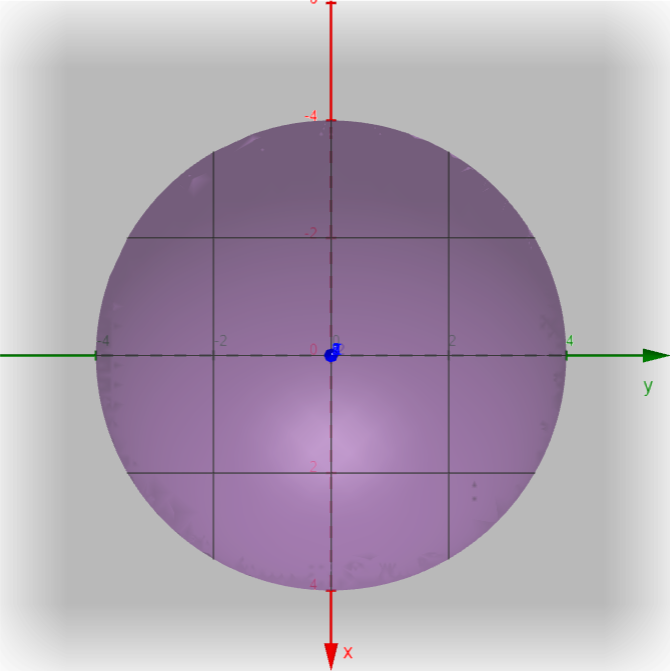
\includegraphics[width=0.35\textwidth]{grafica.1.png}
\vspace{0.5cm}
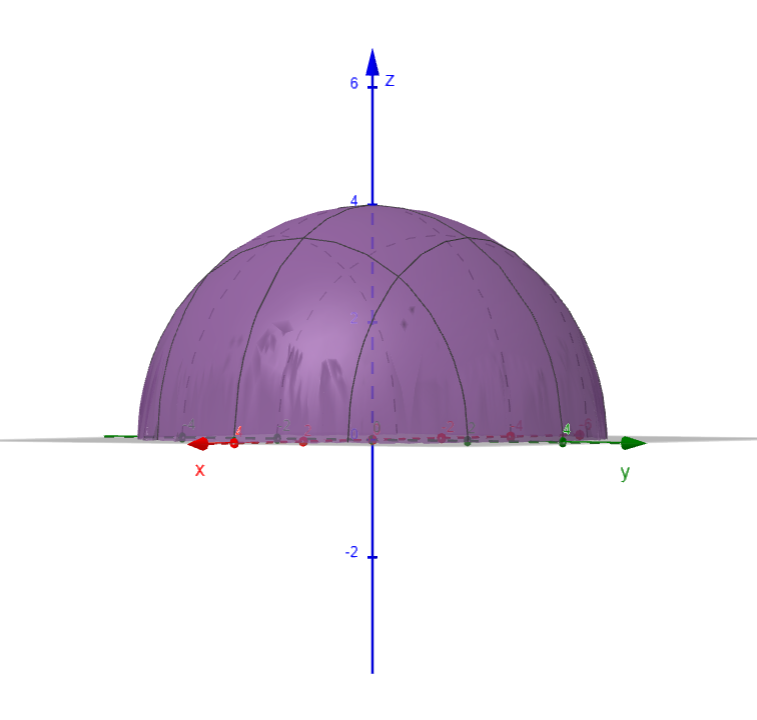
\includegraphics[width=0.35\textwidth]{grafica2.png}
\vspace{0.5cm}
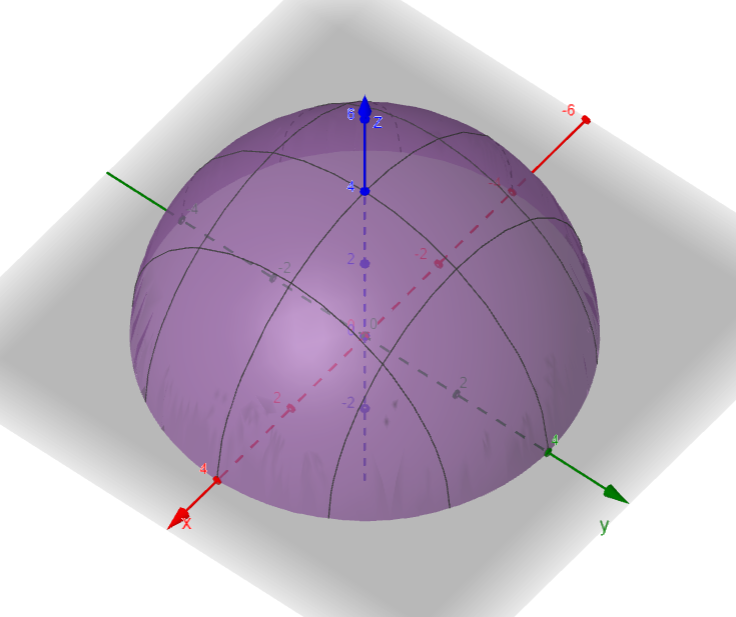
\includegraphics[width=0.3\textwidth]{grafica3.png}
\end{center}
\end{justify}

\newpage

\begin{justify}
{\Large \textbf{Ejercicio 2: Latencia en un Servidor de Metaverso (Función Racional)}}
\vspace{0.1cm}
\[\textbf{Función:}\quad L(d,c)=\frac{d}{100-c}\]

\begin{justify}
{\textbf{1. Variables Independientes:}} {\small d, c}
\vspace{0.01cm}
\end{justify}

\begin{justify}
{\textbf{2. Variables Dependientes:}} {\small L}
\vspace{0.01cm}
\end{justify}

\begin{justify}
{\textbf{3. Dominio:}} {\small 0}
\vspace{0.01cm}
\end{justify}

\begin{center}
\[100-c=0 \quad \Longrightarrow \quad 0 \leq c < 100 \quad \Longrightarrow \quad d=0\]
\end{center}

\begin{justify}
{\textbf{4. Rango:}} \small(0, \infty )
\vspace{0.01cm}
\end{justify}

\begin{center}
\[d \geq 0 \quad \Longrightarrow \quad 100-c > 0 \quad L\geq 0 \quad \Longrightarrow \quad r=(0, \infty)\]
\end{center}

\begin{justify}
    {\textbf{5.¿Cuando es menor la latencia?}}\quad \small Cuando la distancia y la carga sean menor, la latencia tambien sera menor. Ejemplo:
    \vspace{0.01cm}
\end{justify}

\begin{center}
    \[ L= \frac{10}{90}= 0.111\]
\end{center}

\begin{justify}
   {\textbf{6. Tres formas de representacion:}}
   \vspace{0.01cm}
\end{justify}

\begin{justify}
    \small\textbf {Algebraica: } \small
\[L(d,c)=\frac{d}{100-c}\]
\end{justify}

\begin{justify}
\small\textbf {Tabular: }
\begin{tabular}{|c|c|c|}
\hline
\textbf{$d$} & \textbf{$c$} & \textbf{$L$} \\ \hline
10 & 0 & 0.10 \\ \hline
20 & 0 & 0.20 \\ \hline
10 & 50 & 0.20 \\ \hline
20 & 50 & 0.40 \\ \hline
10 & 90 & 1 \\ \hline
20 & 90 & 2 \\ \hline
\end{tabular}
\end{justify}

\begin{justify}
\small\textbf {Grafica: }
\end{justify}

\begin{center}
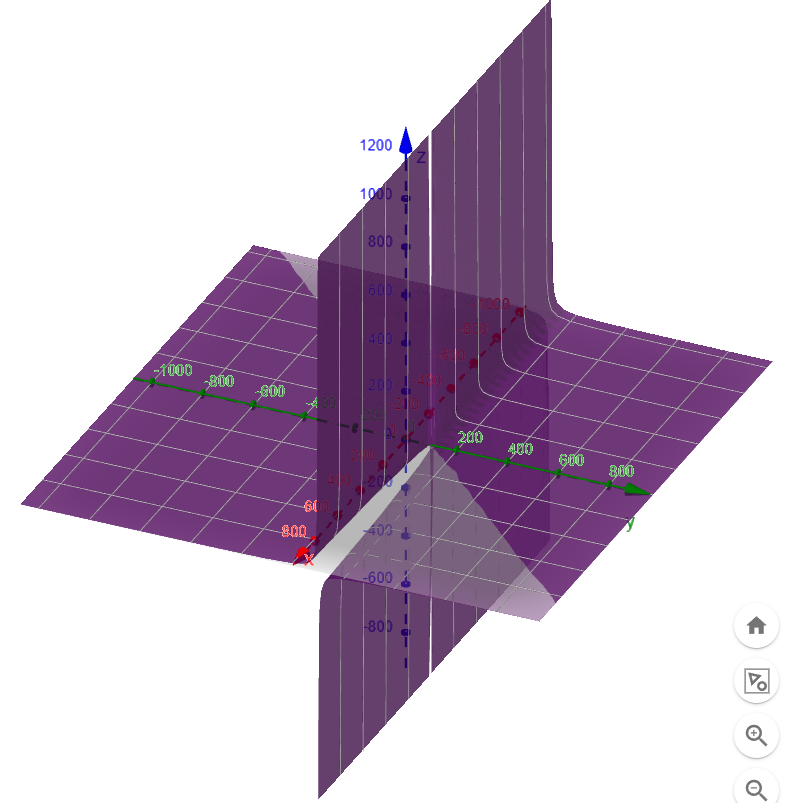
\includegraphics[width=0.3\textwidth]{ejerciciog1.png}
\vspace{0.5cm}
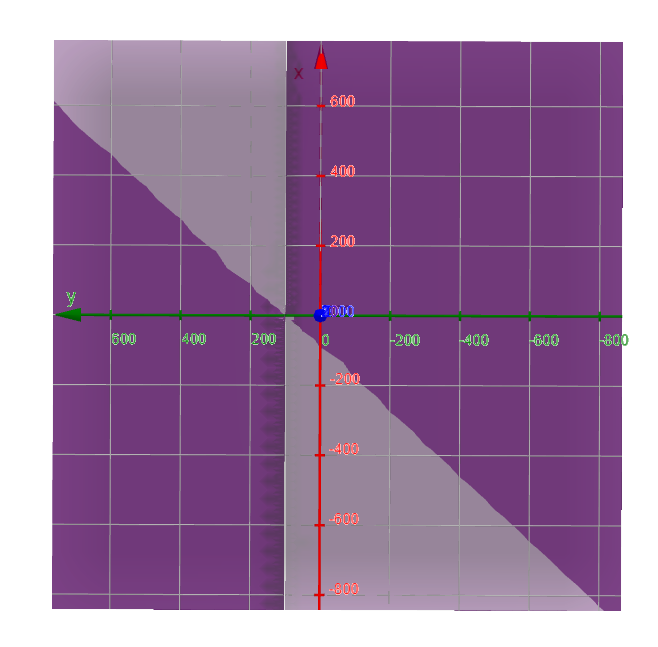
\includegraphics[width=0.3\textwidth]{ejerciciog2.png}
\vspace{0.5cm}
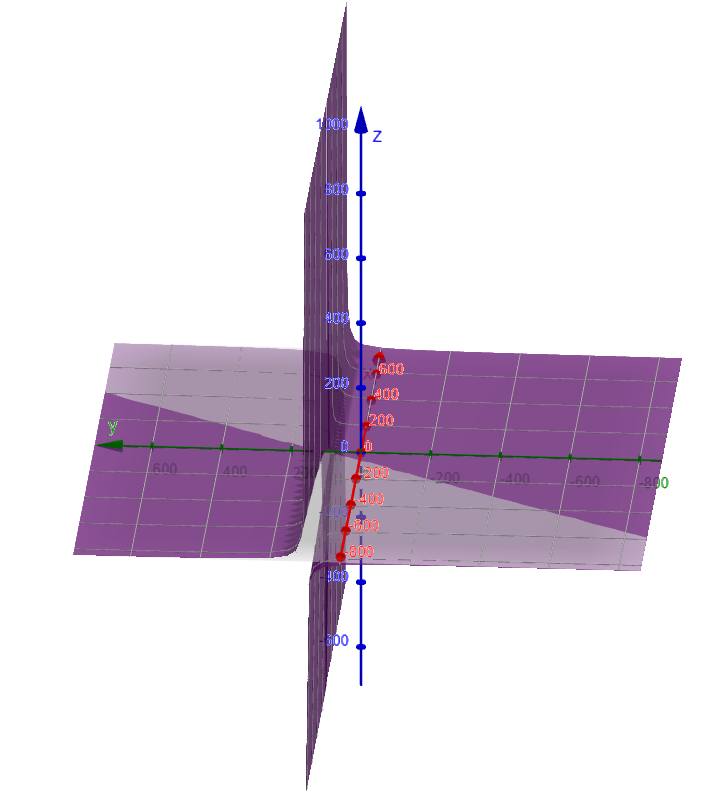
\includegraphics[width=0.3\textwidth]{ejerciciog3.png}
\end{center}

\newpage

\begin{justify}
{\Large \textbf{Ejercicio 3: El Balanceador de Carga (Función Racional)}}
\vspace{0.1cm}
\[\textbf{Función:} \quad f(x,y)=\frac{100}{x+y}\]

\begin{justify}
{\textbf{1. Variables Independientes:}} {\small x, y}
\vspace{0.01cm}
\end{justify}

\begin{justify}
{\textbf{2. Variables Dependientes:}} {\small f(x,y)}
\vspace{0.01cm}
\end{justify}

\begin{justify}
{\textbf{3. Dominio:}} {\small 0}
\vspace{0.01cm}
\end{justify}

\begin{center}
\[x\leq 0 \quad y\leq 0\]
\end{center}

\begin{justify}
{\textbf{4. Rango:}} \small(0, \infty ) \quad 
\vspace{0.01cm}
\end{justify}

\begin{justify}
    \small La carga puede hacercarse a 0 pero no ser solo 0.
\end{justify}

\begin{justify}
    {\textbf{5.¿Cuando es menor la carga?}}\quad \small Cuando la x y y son mayores, la carga se hara menor. Ejemplo:
    \vspace{0.01cm}
\end{justify}

\begin{center}
    \[ x - y = 1000 \quad \Longrightarrow \quad  0.1\]
\end{center}

\begin{justify}
   {\textbf{6. Tres formas de representacion:}}
   \vspace{0.01cm}
\end{justify}

\begin{justify}
    \small\textbf {Algebraica: } \small
\[f(x,y)=\frac{100}{x+y}\]
\end{justify}

\begin{justify}
\small\textbf {Tabular: }
\begin{tabular}{|c|c|c|}
\hline
\textbf{$x$} & \textbf{$y$} & \textbf{$f$} \\ \hline
10 & 10 & 5 \\ \hline
20 & 20 & 2.5 \\ \hline
50 & 50 & 1 \\ \hline
100 & 100 & 0.5 \\ \hline
\end{tabular}
\end{justify}

\begin{justify}
\small\textbf {Grafica: }
\end{justify}

\begin{center}
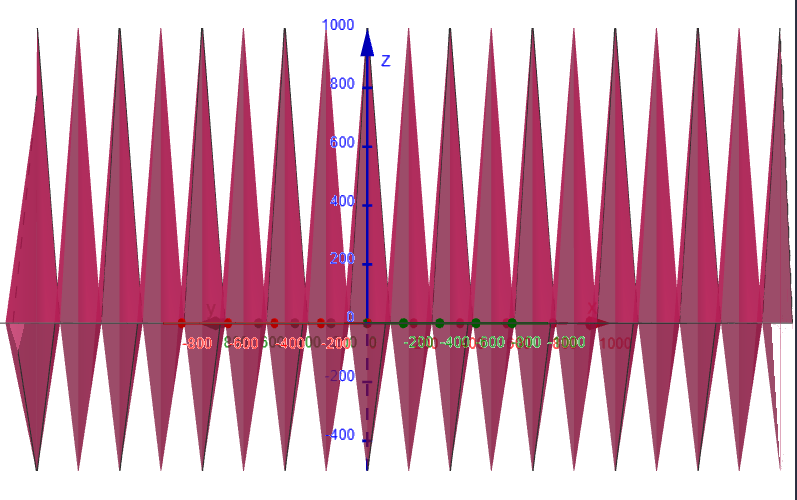
\includegraphics[width=0.3\textwidth]{ejercicio3g1.png}
\vspace{0.5cm}
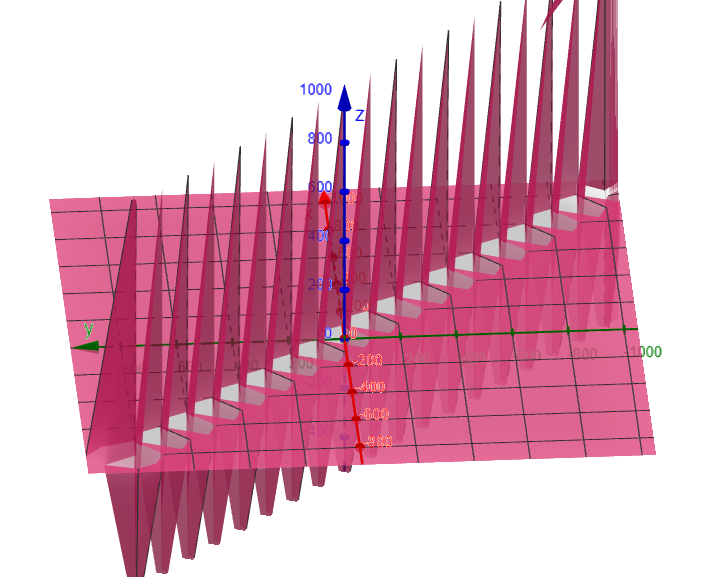
\includegraphics[width=0.3\textwidth]{ejercicio3g2.png}
\vspace{0.5cm}
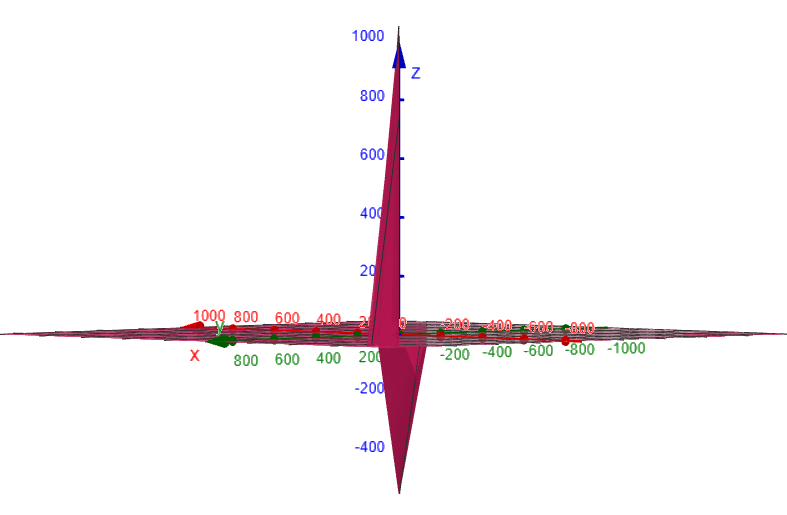
\includegraphics[width=0.3\textwidth]{ejercicio3g3.png}
\end{center}

\newpage

\begin{justify}
{\Large \textbf{Ejercicio 4: Calidad de Experiencia (QoE) en VR (Función de Raíz)}}
\vspace{0.1cm}
\[\textbf{Función:}\quad Q(r, p)=\sqrt{r*p}\]

\begin{justify}
{\textbf{1. Variables Independientes:}} {\small r, p}
\vspace{0.01cm}
\end{justify}

\begin{justify}
{\textbf{2. Variables Dependientes:}} {\small Q(r,p)}
\vspace{0.01cm}
\end{justify}

\begin{justify}
{\textbf{3. Dominio:}} {\small 0}
\vspace{0.01cm}
\end{justify}

\begin{center}
\[r\leq 0 \quad p\leq 0\]
\end{center}

\begin{justify}
{\textbf{4. Rango:}} \small(0, \infty ) \quad 
\vspace{0.01cm}
\end{justify}

\begin{justify}
    \small Puede llegar a 0 si r=0 y p=0.
\end{justify}

\begin{justify}
    {\textbf{5.¿Donde es mayor la calidad?}}\quad \small Cuando la r y la p aumentan, la Q tambien se hace mayor. Ejemplo:
    \vspace{0.01cm}
\end{justify}

\begin{center}
    \[ r=9 \quad p=9 \quad \Longrightarrow \quad  Q= \sqrt{81}=9\]
\end{center}

\begin{justify}
   {\textbf{6. Tres formas de representacion:}}
   \vspace{0.01cm}
\end{justify}

\begin{justify}
    \small\textbf {Algebraica: } \small
\[Q=\sqrt{rp}\]
\end{justify}

\begin{justify}
\small\textbf {Tabular: }
\begin{tabular}{|c|c|c|}
\hline
\textbf{$r$} & \textbf{$p$} & \textbf{$Q$} \\ \hline
1 & 1 & 1 \\ \hline
2 & 2 & 2 \\ \hline
4 & 4 & 4 \\ \hline
9 & 4 & 6 \\ \hline
16 & 9 & 12 \\ \hline
\end{tabular}
\end{justify}

\begin{justify}
\small\textbf {Grafica: }
\end{justify}

\begin{center}
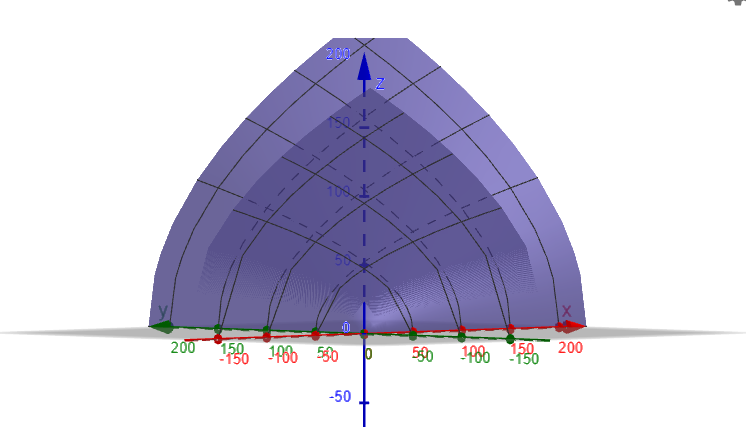
\includegraphics[width=0.3\textwidth]{ejercicio4g1.png}
\vspace{0.5cm}
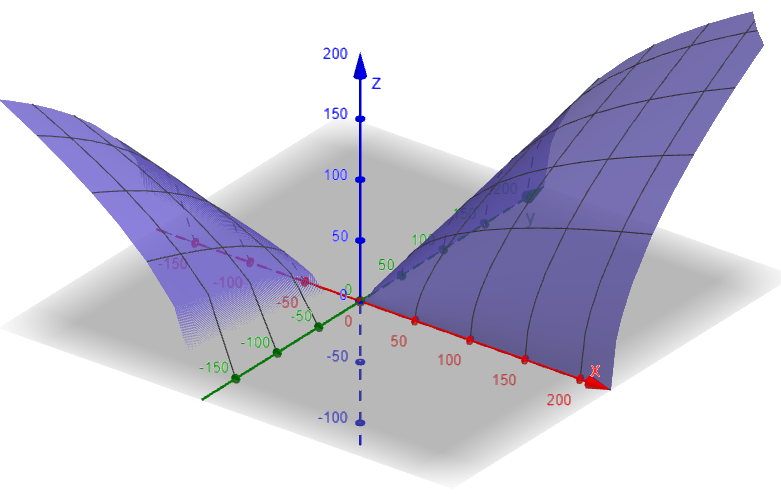
\includegraphics[width=0.3\textwidth]{ejercicio4g2.png}
\vspace{0.5cm}
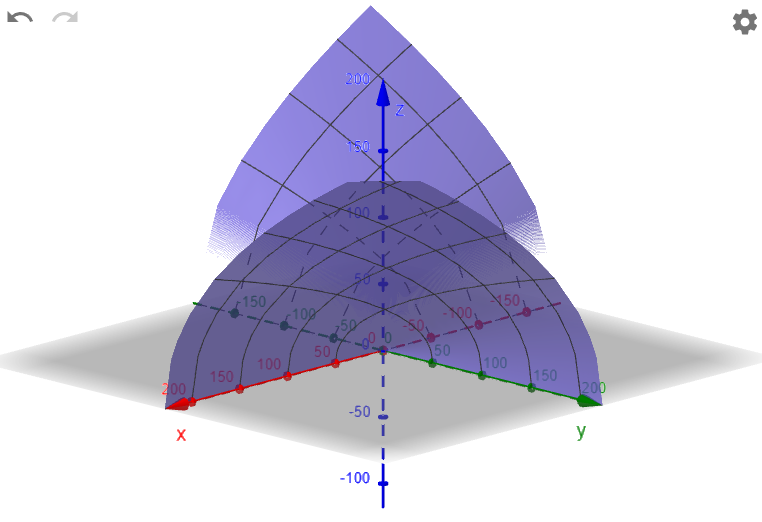
\includegraphics[width=0.3\textwidth]{ejercicio4g3.png}
\end{center}

\newpage

\begin{justify}
{\Large \textbf{Ejercicio 5: Algoritmo Logarítmico (Restricción de Logaritmo)}}
\vspace{0.1cm}
\[\textbf{Función:}\quad f(x,y) = In(y-x^2)\]

\begin{justify}
{\textbf{1. Variables Independientes:}} {\small x, y}
\vspace{0.01cm}
\end{justify}

\begin{justify}
{\textbf{2. Variables Dependientes:}} {\small f(x,y)}
\vspace{0.01cm}
\end{justify}

\begin{justify}
{\textbf{3. Dominio:}} {\small y > x^2}
\vspace{0.01cm}
\end{justify}

\begin{center}
\[y-x^2>0 \quad \Longrightarrow \quad y>x^2 \]
\end{center}

\begin{justify}
{\textbf{4. Rango:}} \smallCualquier numero positivo puede producir un numero real. \quad 
\vspace{0.01cm}
\end{justify}

\begin{justify}
   {\textbf{6. Tres formas de representacion:}}
   \vspace{0.01cm}
\end{justify}

\begin{justify}
    \small\textbf {Algebraica: } \small
\[f(x,y) = In(y-x^2)\]
\end{justify}

\begin{justify}
\small\textbf {Tabular: }
\begin{tabular}{|c|c|c|}
\hline
\textbf{$x$} & \textbf{$y$} & \textbf{$In(y-x^2)$} \\ \hline
0 & 1 & In(1)=0 \\ \hline
0 & 2 & In(2)=0.69 \\ \hline
1 & 2 & In(1)=0 \\ \hline
1 & 3 & In(2)=0.69 \\ \hline
2 & 5 & In(1)=0 \\ \hline
2 & 6 & In(2)=0.69 \\ \hline
\end{tabular}
\end{justify}

\begin{justify}
\small\textbf {Grafica: }
\end{justify}

\begin{center}
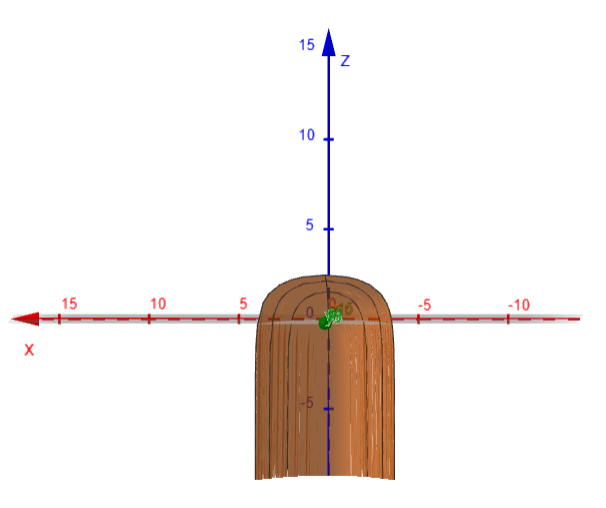
\includegraphics[width=0.4\textwidth]{ejercicio5g1.png}
\vspace{0.5cm}
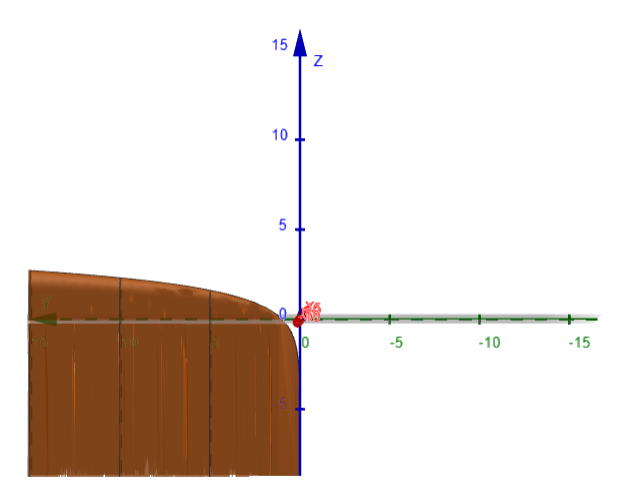
\includegraphics[width=0.4\textwidth]{ejercicio5g2.png}
\vspace{0.5cm}
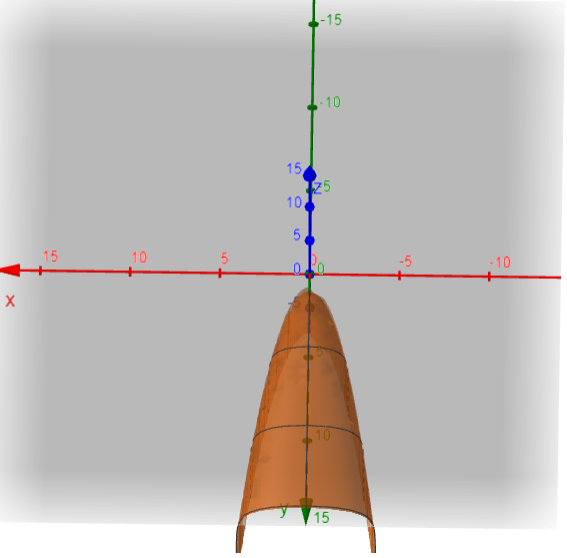
\includegraphics[width=0.4\textwidth]{ejercicio5g3.png}
\end{center}

\newpage

\begin{justify}
{\Large \textbf{Ejercicio 6: Utilidad Neta de un Producto Digital (Función Logarítmica)}}
\vspace{0.1cm}
\[\textbf{Función:}\quad u(v, g) = In(v-g)\]

\begin{justify}
{\textbf{1. Variables Independientes:}} {\small v, g}
\vspace{0.01cm}
\end{justify}

\begin{justify}
{\textbf{2. Variables Dependientes:}} {\small u}
\vspace{0.01cm}
\end{justify}

\begin{justify}
{\textbf{3. Dominio:}} {\small v > g}
\vspace{0.01cm}
\end{justify}

\begin{center}
\[v-g>0 \quad \Longrightarrow \quad v>g \]
\end{center}

\begin{justify}
{\textbf{4. Rango:}} \smallCualquier (-\infty, \infty) . \quad  
\vspace{0.01cm}
\end{justify}

\begin{justify}
    \small Puede tomar cualquier valor positivo. 
\end{justify}

\begin{justify}
    {\textbf{5.¿Donde es mayor la unidad?}}\quad \small Cuando la r y la p aumentan, la Q tambien se hace mayor. Ejemplo:
    \vspace{0.01cm}
\end{justify}

\begin{justify}
   {\textbf{6. Tres formas de representacion:}}
   \vspace{0.01cm}
\end{justify}

\begin{justify}
    \small\textbf {Algebraica: } \small
\[u(v,g) = In(v-g)\]
\end{justify}

\begin{justify}
\small\textbf {Tabular: }
\begin{tabular}{|c|c|c|c|}
\hline
\textbf{$v$} & \textbf{$g$} & \textbf{$v-g$} & \textbf{$u=In(v-g)$} \\ \hline
10 & 5 & 5 & 1.61 \\ \hline
20 & 10 & 10 & 2.30\\ \hline
20 & 15 & 5 & 1.61\\ \hline
20 & 19 & 1 & 0\\ \hline
30 & 20 & 10 & 2.30\\ \hline
\end{tabular}
\end{justify}

\begin{justify}
\small\textbf {Grafica: }
\end{justify}

\begin{center}
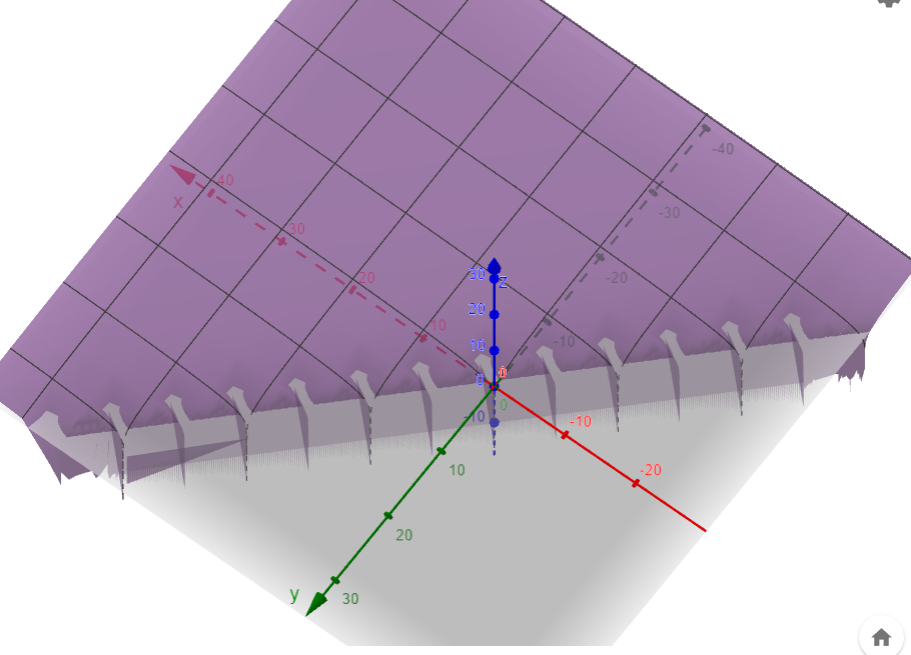
\includegraphics[width=0.4\textwidth]{ejercicio6g1.png}
\vspace{0.5cm}
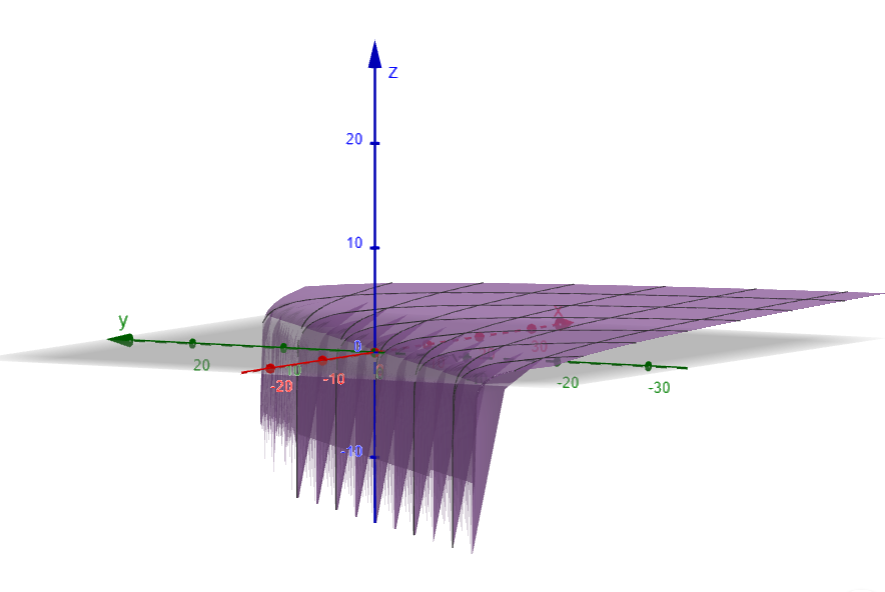
\includegraphics[width=0.4\textwidth]{ejercicio6g2.png}
\vspace{0.5cm}
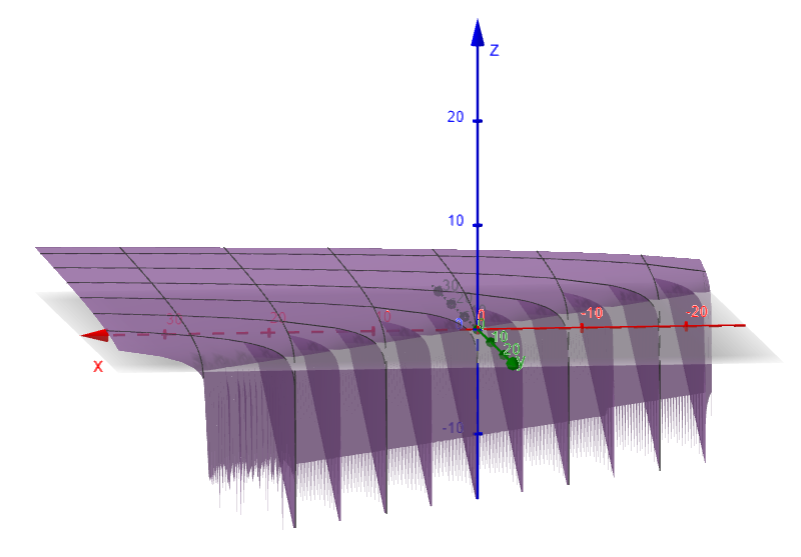
\includegraphics[width=0.4\textwidth]{ejercicio6g3.png}
\end{center}

\newpage

\begin{justify}
{\Large \textbf{Ejercicio 7:El Filtro de Ruido Gaussiano (Exponencial)}}
\vspace{0.1cm}
\[\textbf{Función:}\quad f(x,y) = e^{-(x^2+y^2)\]

\begin{justify}
{\textbf{1. Variables Independientes:}} {\small x, y}
\vspace{0.01cm}
\end{justify}

\begin{justify}
{\textbf{2. Variables Dependientes:}} {\small f(x,y)}
\vspace{0.01cm}
\end{justify}

\begin{justify}
{\textbf{3. Dominio:}} {\small - \infty < x < \infty \quad -\infty < y < \infty}
\vspace{0.01cm}
\end{justify}

\begin{justify}
    \small Se puede utilizar cualquier valor en x y y.
\end{justify}

\begin{justify}
{\textbf{4. Rango:}} \smallCualquier (0, 1) . \quad  
\vspace{0.01cm}
\end{justify}

\begin{justify}
    \[ f(0,0) = e^{-(0^2+0^2)} \quad \Longrightarrow \quad = e^0 \quad \Longrightarrow \quad = 1\]
\end{justify}

\begin{justify}
   {\textbf{5. Tres formas de representacion:}}
   \vspace{0.01cm}
\end{justify}

\begin{justify}
    \small\textbf {Algebraica: } \small
\[f(x,y) = e^{-(x^2 + y^2)}\]
\end{justify}

\begin{justify}
\small\textbf {Tabular: }
\begin{tabular}{|c|c|c|}
\hline
\textbf{$x$} & \textbf{$y$} & \textbf{$f(x,y)$} \\ \hline
0 & 0 & 1 \\ \hline
1 & 0 & 0.368 \\ \hline
0 & 1 & 1.368 \\ \hline
1 & 1 & 0.135 \\ \hline
2 & 0 & 0.018 \\ \hline
\end{tabular}
\end{justify}

\begin{justify}
\small\textbf {Grafica: }
\end{justify}

\begin{center}
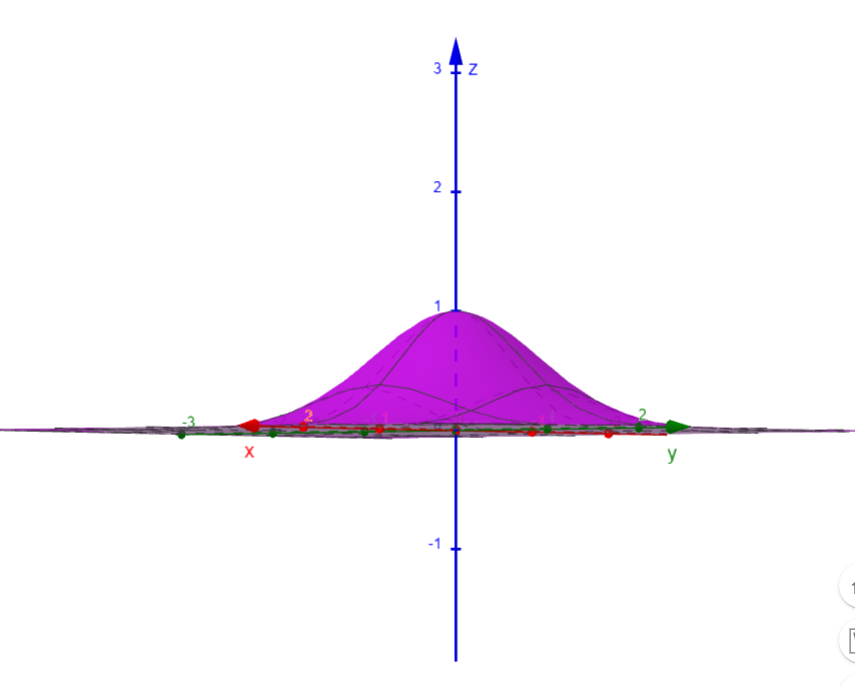
\includegraphics[width=0.4\textwidth]{ejercicio7g1.png}
\vspace{0.5cm}
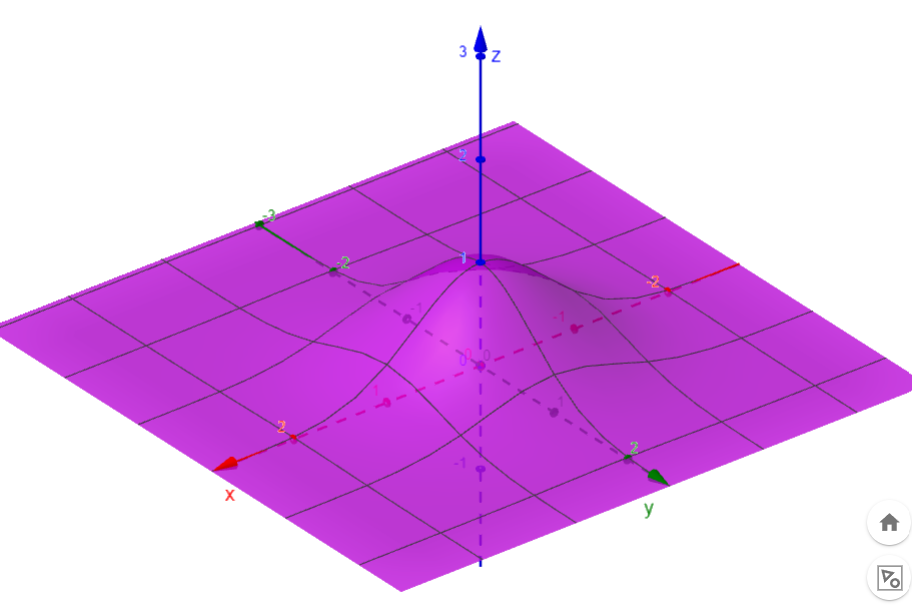
\includegraphics[width=0.4\textwidth]{ejercicio7g2.png}
\vspace{0.5cm}
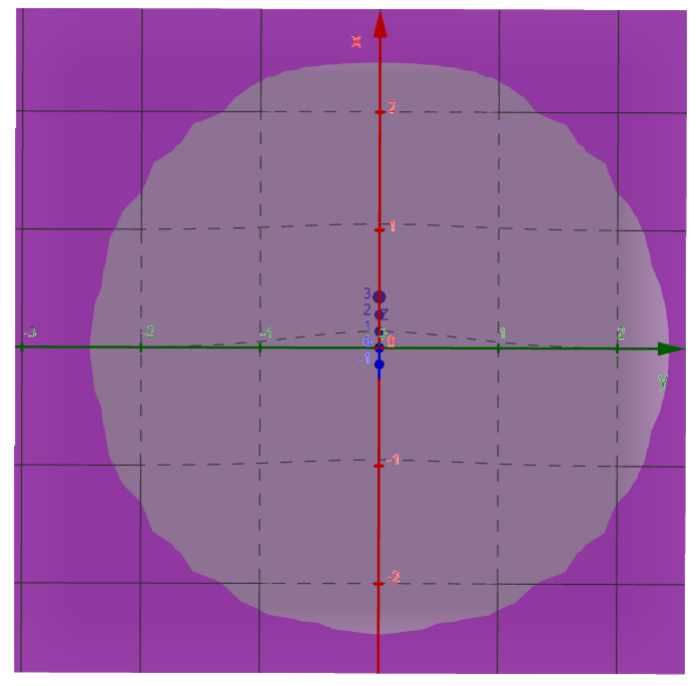
\includegraphics[width=0.4\textwidth]{ejercicio7g3.png}
\end{center}

\newpage

\begin{justify}
{\Large \textbf{Ejercicio 8: Zona de Seguimiento (Tracking) en VR (Paraboloide)}}
\vspace{0.1cm}
\[\textbf{Función:}\quad Z(x,y) = x^2+y^2\]

\begin{justify}
{\textbf{1. Variables Independientes:}} {\small x, y}
\vspace{0.01cm}
\end{justify}

\begin{justify}
{\textbf{2. Variables Dependientes:}} {\small Z(x,y)}
\vspace{0.01cm}
\end{justify}

\begin{justify}
{\textbf{3. Dominio:}} {\small Se puede utilizar cualquier numero real para x y y.}
\vspace{0.01cm}
\end{justify}

\begin{justify}
{\textbf{4. Rango:}} \small (0, \infty) 
\vspace{0.01cm}
\end{justify}

\begin{justify}
    \[ x^2+y^2 \leq 0 \quad \Longrightarrow \quad Z=0^2+0^2 \]
\end{justify}

\begin{justify}
   {\textbf{5. Tres formas de representacion:}}
   \vspace{0.01cm}
\end{justify}

\begin{justify}
    \small\textbf {Algebraica: } \small
\[Z(x,y) = x^2+y^2\]
\end{justify}

\begin{justify}
\small\textbf {Tabular: }
\begin{tabular}{|c|c|c|}
\hline
\textbf{$x$} & \textbf{$y$} & \textbf{$Z$} \\ \hline
0 & 0 & 0 \\ \hline
1 & 0 & 1 \\ \hline
0 & 1 & 1 \\ \hline
1 & 1 & 2 \\ \hline
2 & 2 & 8 \\ \hline
\end{tabular}
\end{justify}

\begin{justify}
\small\textbf {Grafica: }
\end{justify}

\begin{center}
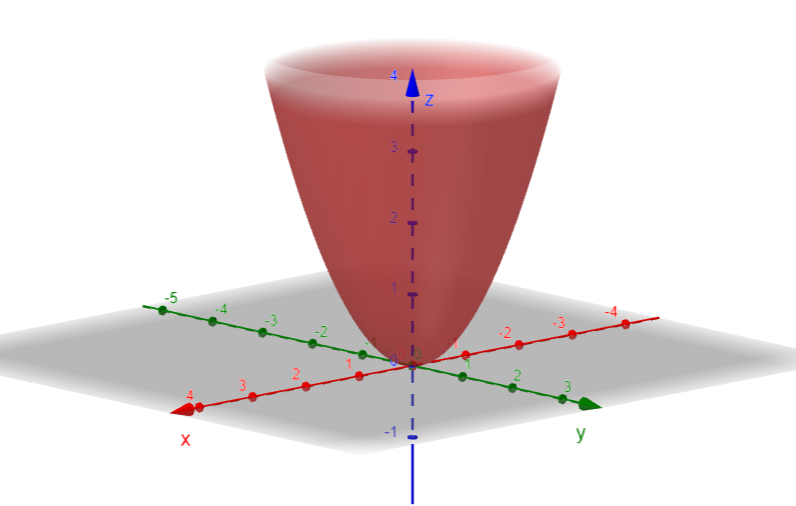
\includegraphics[width=0.4\textwidth]{ejercicio8g1.png}
\vspace{0.5cm}
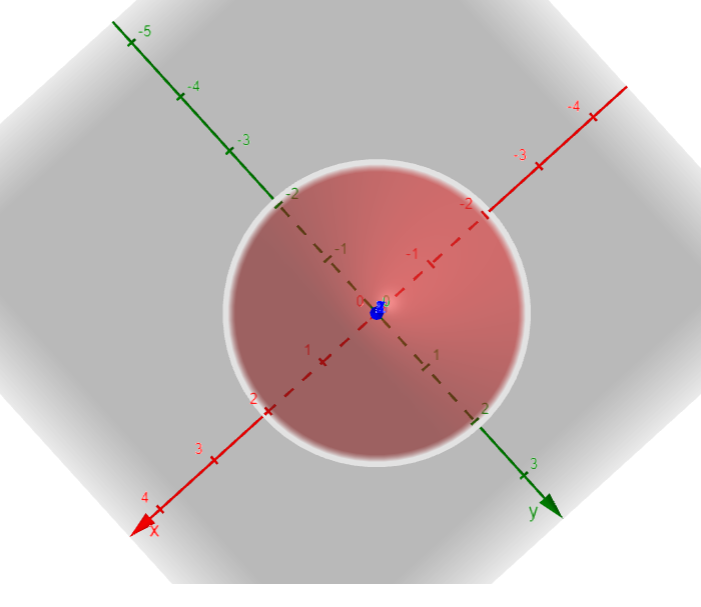
\includegraphics[width=0.4\textwidth]{ejercicio8g2.png}
\vspace{0.5cm}
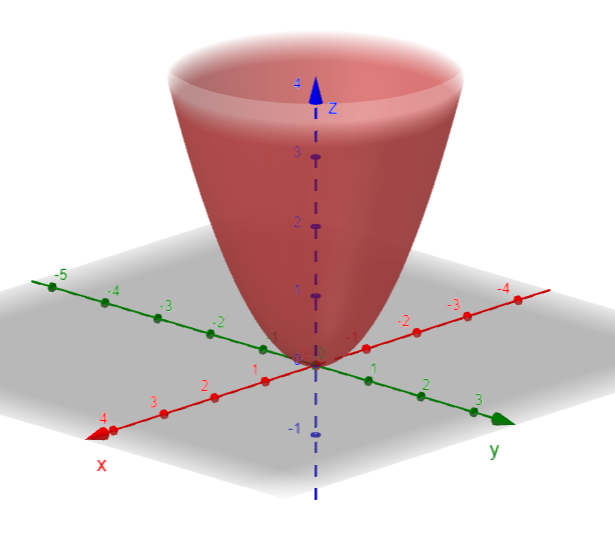
\includegraphics[width=0.4\textwidth]{ejercicio8g3.png}
\end{center}

\newpage

\begin{justify}
{\Large \textbf{Ejercicio 9:: El Costo de Almacenamiento (Suma de Raíces).}}
\vspace{0.1cm}
\[\textbf{Función:}\quad f(x,y) = \sqrt{x}+\sqrt{y}\]

\begin{justify}
{\textbf{1. Variables Independientes:}} {\small x, y}
\vspace{0.01cm}
\end{justify}

\begin{justify}
{\textbf{2. Variables Dependientes:}} {\small f(x,y)}
\vspace{0.01cm}
\end{justify}

\begin{justify}
{\textbf{3. Dominio:}} {\small x\leq 0, y\quad 0}
\vspace{0.01cm}
\end{justify}

\begin{justify}
{\textbf{4. Rango:}} \small (0, \infty) 
\vspace{0.01cm}
\end{justify}

\begin{justify}
    \[ f(x,y) \leq 0 \quad \Longrightarrow \quad x=0, \quad y=0 \]
\end{justify}

\begin{justify}
   {\textbf{5. Tres formas de representacion:}}
   \vspace{0.01cm}
\end{justify}

\begin{justify}
    \small\textbf {Algebraica: } \small
\[f(x,y) = \sqrt{x}+\sqrt{y}\]
\end{justify}

\begin{justify}
\small\textbf {Tabular: }
\begin{tabular}{|c|c|c|}
\hline
\textbf{$x$} & \textbf{$y$} & \textbf{$Z$} \\ \hline
0 & 0 & 0 \\ \hline
1 & 1 & 2 \\ \hline
4 & 1 & 3 \\ \hline
1 & 9 & 4 \\ \hline
4 & 4 & 4 \\ \hline
\end{tabular}
\end{justify}

\begin{justify}
\small\textbf {Grafica: }
\end{justify}

\begin{center}
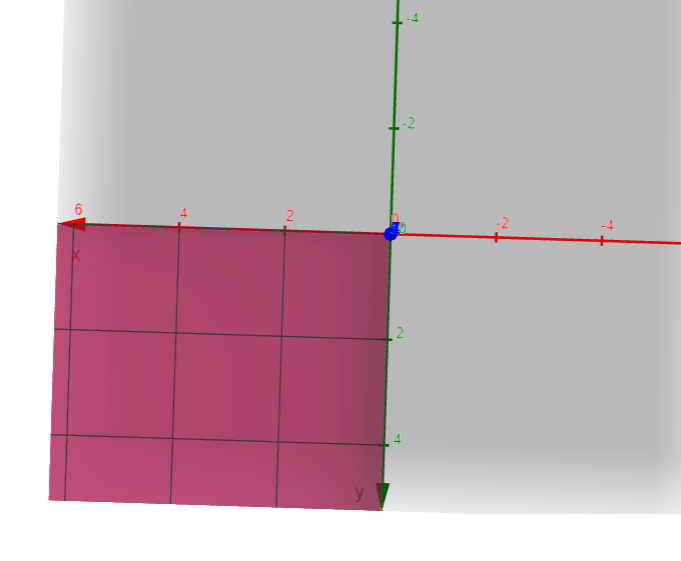
\includegraphics[width=0.4\textwidth]{ejercicio9g1.png}
\vspace{0.5cm}
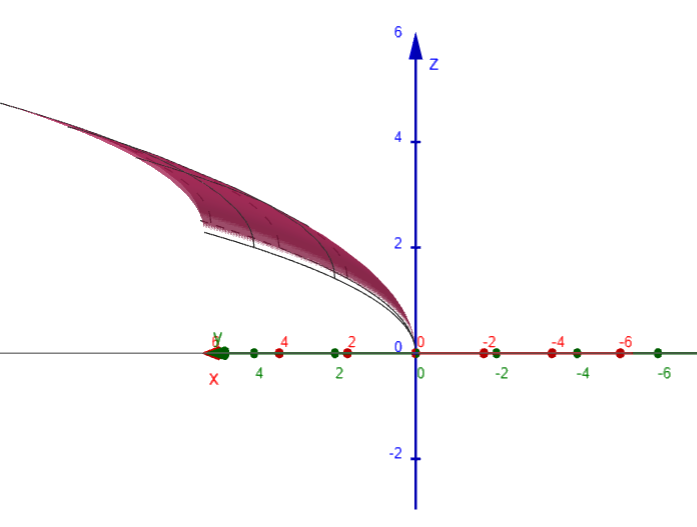
\includegraphics[width=0.4\textwidth]{ejercicio9g2.png}
\vspace{0.5cm}
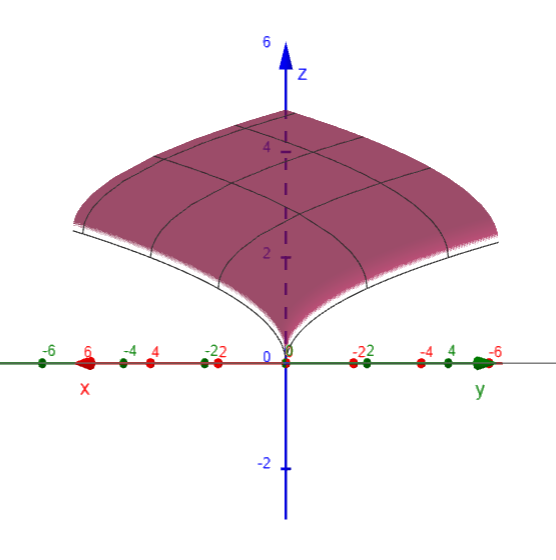
\includegraphics[width=0.4\textwidth]{ejercicio9g3.png}
\end{center}

\newpage

\begin{justify}
{\Large \textbf{Ejercicio 10:: Tasa de Conversión en E-commerce (Función Exponencial).}}
\vspace{0.1cm}
\[\textbf{Función:}\quad t(u,s) = 1 - e^{-(u+s)}\]

\begin{justify}
{\textbf{1. Variables Independientes:}} {\small u, s}
\vspace{0.01cm}
\end{justify}

\begin{justify}
{\textbf{2. Variables Dependientes:}} {\small T(u,s)}
\vspace{0.01cm}
\end{justify}

\begin{justify}
{\textbf{3. Dominio:}} {\small u\leq 0, s\quad 0}
\vspace{0.01cm}
\end{justify}

\begin{justify}
{\textbf{4. Rango:}} \small (0, 1) 
\vspace{0.01cm}
\end{justify}

\begin{justify}
    
\end{justify}
\[ u=0 \quad s=0 \quad \Longrightarrow \quad T=1-e^0 \quad \Longrightarrow \quad T=1-1  \quad \Longrightarrow \quad T=0 \]
\begin{justify}
 \[ e^{-(u+s)}=0 \quad \Longrightarrow \quad T=1 \]
\end{justify}

\begin{justify}
   {\textbf{5. Tres formas de representacion:}}
   \vspace{0.01cm}
\end{justify}

\begin{justify}
    \small\textbf {Algebraica: } \small
\[t(u,s) = 1 - e^{-(u+s)}\]
\end{justify}

\begin{justify}
\small\textbf {Tabular: }
\begin{tabular}{|c|c|c|}
\hline
\textbf{$x$} & \textbf{$y$} & \textbf{$Z$} \\ \hline
0 & 0 & 0 \\ \hline
1 & 0 & 0.632 \\ \hline
0 & 1 & 0.632 \\ \hline
1 & 1 & 0.865 \\ \hline
2 & 1 & 0.950 \\ \hline
2 & 2 & 0.982 \\ \hline
\end{tabular}
\end{justify}

\begin{justify}
\small\textbf {Grafica: }
\end{justify}

\begin{center}
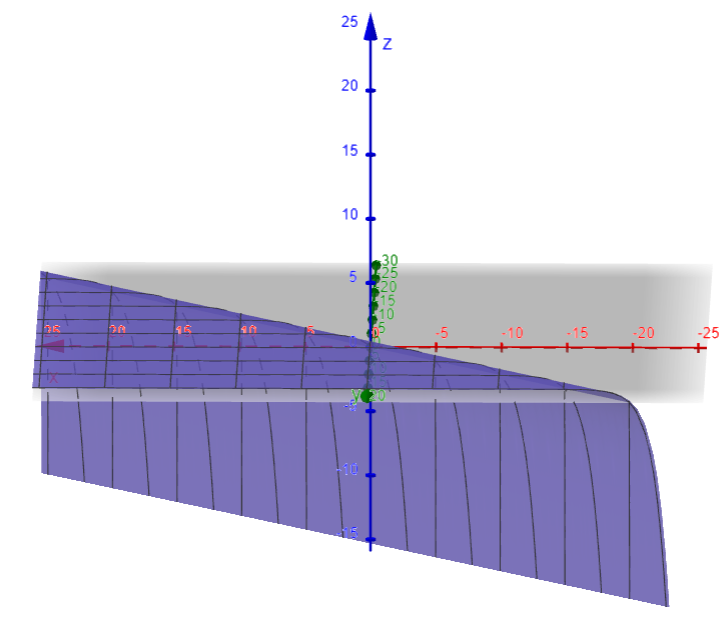
\includegraphics[width=0.4\textwidth]{ejercicio10g1.png}
\vspace{0.5cm}
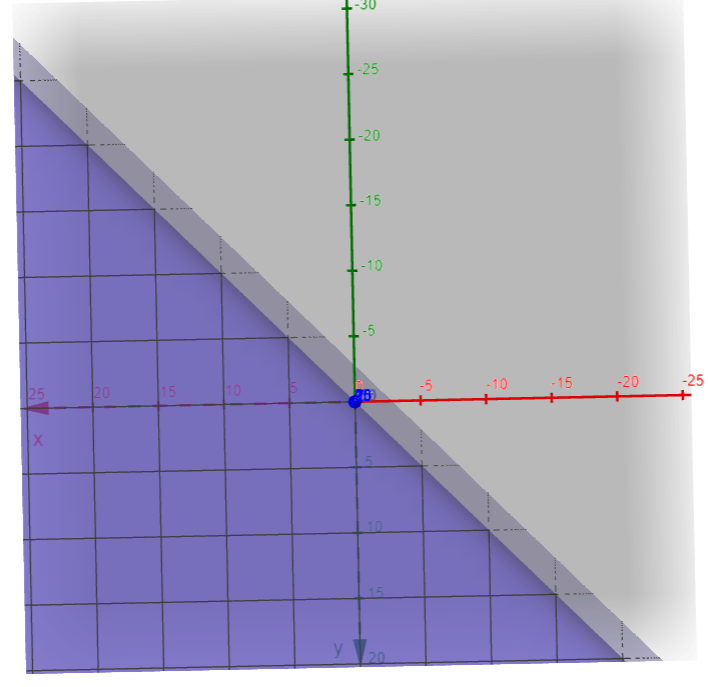
\includegraphics[width=0.4\textwidth]{ejercicio10g2.png}
\vspace{0.5cm}
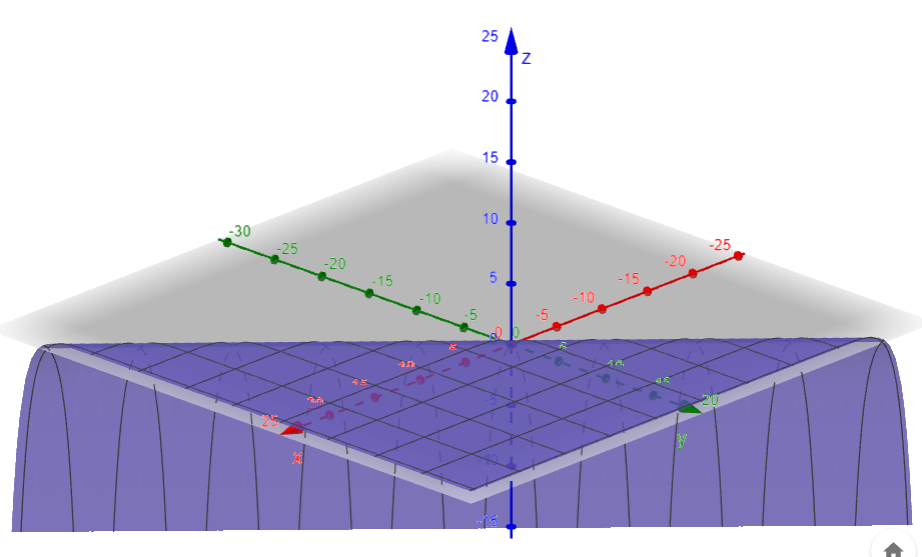
\includegraphics[width=0.4\textwidth]{ejercicio10g3.png}
\end{center}

\end{justify}
\end{document}